\documentclass[a4paper, twoside,openright]{report}
\usepackage[T1]{fontenc} % Font encoding, T1 = it
\usepackage[utf8]{inputenc} % Input encoding - per caratteri particolari
\usepackage[english,italian]{babel} % Lingua principale italiano, con parti in inglese
\usepackage{graphicx} % Per includere immagini esterne
\usepackage{lipsum} % genera testo fittizio
\usepackage[a4paper,top=3cm,bottom=3cm,left=3cm,right=3cm]{geometry} %impaginazione e margini documento
\usepackage[fontsize=12pt]{scrextend} %dimensione font
\usepackage{float}

\setlength{\textfloatsep}{10pt}     % Space between text and float
\setlength{\intextsep}{10pt}    

\begin{document}
\input{frontespizio}


\section{Introduction}
Our work is about to analyze and extract a perfect clean data for usage of machine learning training. This work is applied to 2 different datasets: cyclists dataset and race dataset. Sequence of action made for elaborate datasets are:

1) Analyze distribution and correlation between features.
2) Feature engineering for managing missing values

\section{Data understanding}

\subsection{Missing values}
\subsubsection{Scraping}

During the data quality assessment task, we identified three fundamental issues with the races' dataset:
\begin{itemize}

\item (UCI) Points duplication: \\ 
Each cyclist in a particular race received the same number of points,  which were identical to those awarded to the first-place cyclist. 
\item  Incorrect final position: \\
We discovered that some cyclists were disqualified from certain races, yet the dataset retained their original positions unchanged. The substitute and subsequent riders were incorrectly shifted down by one position. \\
Example: If 15th placed rider was disqualified, the replacement one was incorrectly listed in 16th position.
\item Negative deltas: \\
We found out the cause of negative deltas was a different representation of the same value. The first positioned rider has a finishing time, for example, 0:40:00, which stands for the hours, minutes, and seconds needed to arrive as number one. The subsequent ones were given either a positive value, which means the arrived time after the first one, or a negative value, which express the hours, minutes, and seconds required to cross the finishing line, for example: -0:42:00. Therefore, the correct delta was assumed to be 0:42:00–0:40:00 = 2:00.
\end{itemize}

Lastly, one issue with cyclists dataset:
\begin{itemize}
    \item Missing cyclists: \\
    In addition, we realized that some cyclists were only present in the race dataset but not in the cyclist dataset.
\end{itemize}

After careful consideration, we decided to obtain a better version of the two dataset by scraping this website:
\textit{https://www.procyclingstats.com}

\subsection{Correlation between features}
\subsection{Correlation Matrix}

 We begin the feature correlation analysis with the correlation matrix between all the numerical features of the two datasets combined.
\begin{figure}[ht]
    \centering
    \includegraphics[width=0.6\textwidth]{assets/correlation_matrix.png}
    \caption{Correlation matrix between all relevant features.}
    \label{fig:correlation-matrix}
\end{figure}
We observed a strong expected positive correlation between \textit{height} and \textit{weight} (0.74), \textit{climb\_total} and \textit{profile} (0.71), \textit{points} and \textit{uci\_points} (0.84).  In addition, there is a significant positive correlation between  \textit{climb\_total} and  \textit{length} (0.52). Less evident positive correlation is \textit{delta} and \textit{length} (0.25). \\
Regarding the negative correlation, we noted that there is a weak negative correlation between \textit{length} and \textit{is\_tarmac} (0.36), which might indicate that the longer the race, the less likely it is to be primary on tarmac.  As the second most significant negative correlation, we have the one between \textit{points} and \textit{is\_tarmac} (0.32), which again might indicate that a race has more points, on average, the more likely it is to have different types of terrain. Furthermore, there are negative correlations such as \textit{points} and \textit{position} (0.31), \textit{profile} and \textit{delta} (0.28). The last one is counterintuitive, even though it is a feeble correlation, which might indicate that as the race profile becomes more challenging (moving from flat towards high mountains with uphill finish), the time gaps (delta) between riders tend to decrease because of riders grouping?
\subsection{Points, Age, Temperature and Career Span}
Even though the number of available \textit{average\_temperature} samples is limited, it is informative to compare how age groups perform across different temperature ranges.
\begin{figure}[ht]
    \centering
    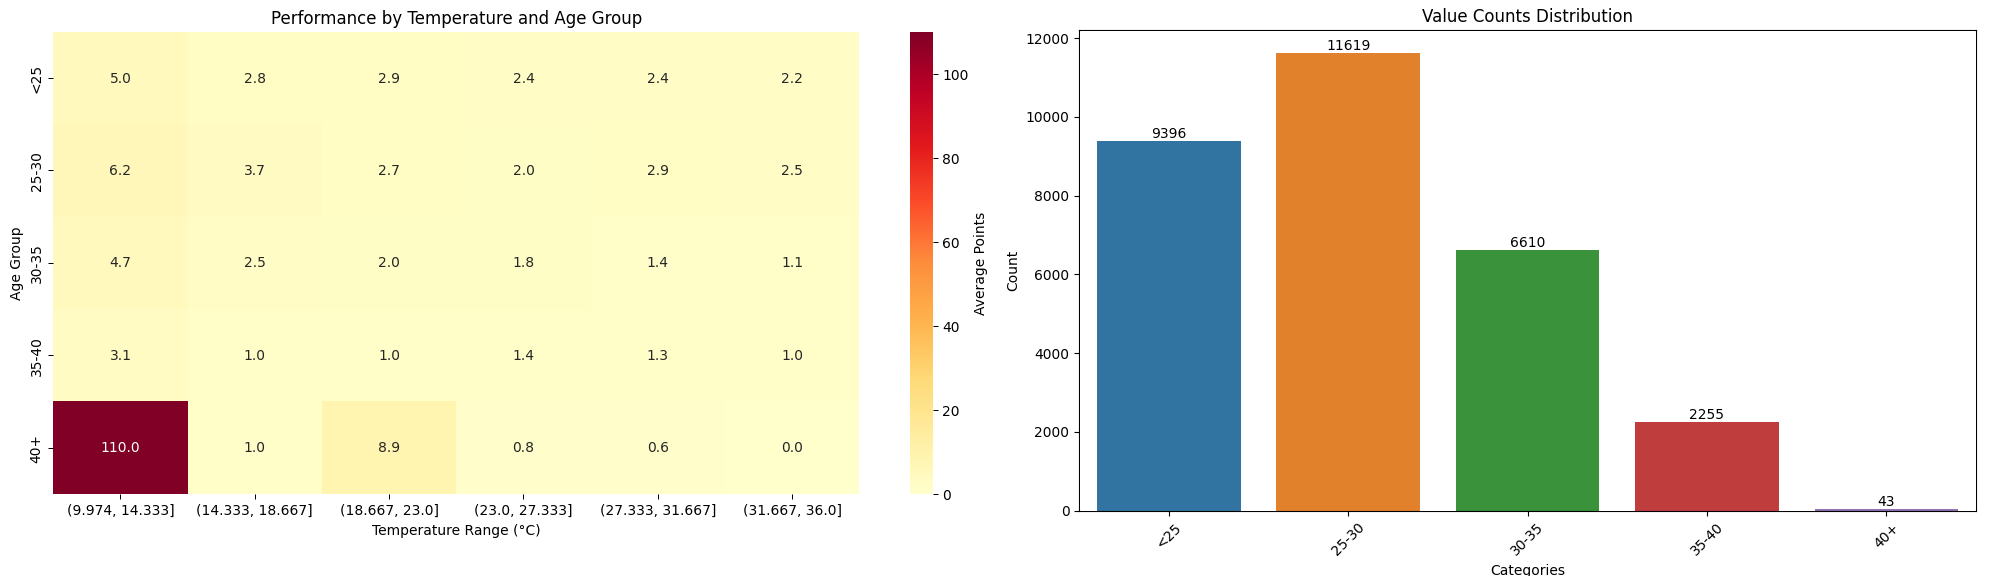
\includegraphics[width=0.55\textwidth]{assets/perf_age_group.png}
    \caption{Average points by age group and temperature range.}
    \label{fig:temperature-age}
\end{figure}
As shown in Figure~\ref{fig:temperature-age}, the 40+ group exhibits high average points (110.0) within the (9.9--14.3) temperature range, and 8.9 points within the (18.6--110.0) range. However, this group has a very small sample size (Figure~\ref{fig:counts_age_group_with_temp}), partly because riders often retire before reaching 40. Consequently, the limited data for this group may skew the average.
\begin{figure}[ht]
    \centering
    \includegraphics[width=0.5\textwidth]{assets/counts_age_group.png}
    \caption{Age distribution of cyclists.}
    \label{fig:counts_age_group_with_temp}
\end{figure}
Next, we examine how age correlates with riders' performance and the cyclists' career duration.
\begin{figure}[ht]
    \centering
    \includegraphics[width=0.6\textwidth]{assets/distributions_rel.png}
    \caption{Average points by age group.}
    \label{fig:points-age}
\end{figure}

\subsection{Correct values check}

\section{Data transformation}

\subsection{Fill missing data}

\subsection{Feature engineering}

\subsection{Outlier detection}

\section{Data clustering}

\subsection{K-means}

\subsection{DBSCAN clustering}

\subsection{Hierarchical clustering}

\section{Predictive models}

\subsection{Linear classification}

\subsection{Neural network}

\subsection{Support vector machine}

\subsection{Autoencoder}

\subsection{Decision tree}

\subsection{Random forest}

\section{Conclusion}
Test cite\cite{test_cite}

\bibliographystyle{plain}
\bibliography{References}

\end{document}